{\fontsize{12pt}{22pt} \textbf{Distribution functions}\par}

\vspace{5mm}

\underline{Mass function}

The probability mass function (p.m.f.) is the histogram of the distribution, that is:

- x-axis: values

- y-axis: frequency

\vspace{5mm}

\underline{Density function}

The probability density function (p.d.f.) is the "smooth histogram" of the distribution.

\vspace{5mm}

\begin{center}
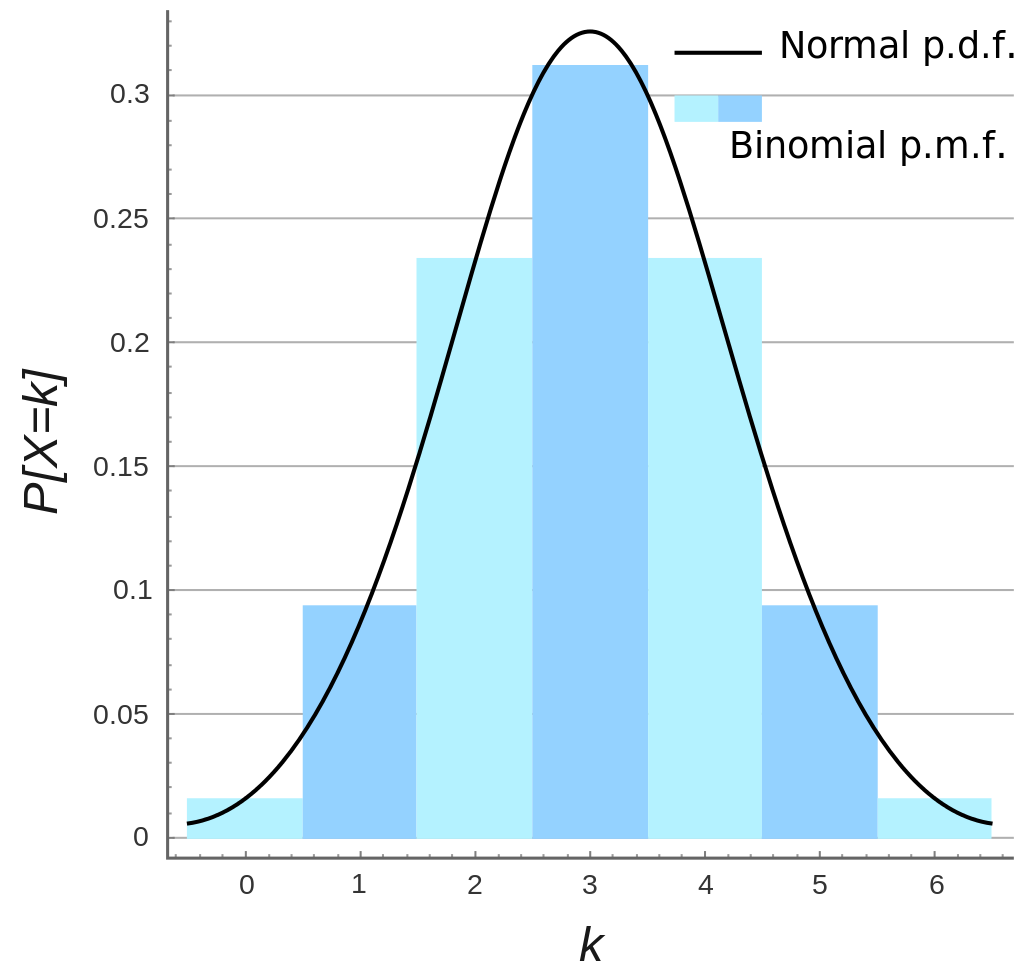
\includegraphics[scale=0.15]{mass_density_functions.png}
\end{center}

\vspace{5mm}

\underline{Cumulative distribution function}

The cumulative distribution function (c.d.f) is given by $F_X(x)= \mathbb{P}(X < x)$. 

The empirical distribution function is its estimation:
$\widehat{F}_n(x) = \frac{1}{n}\{\text{number of elements} < x\}$

\begin{center}
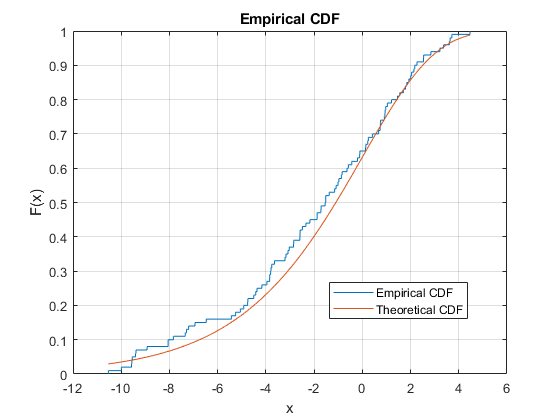
\includegraphics[scale=0.4]{CDF.png}
\end{center}

\lstset{language=Python}
\lstset{frame=lines}
\lstset{caption={Python CDF easy implementation}}
\lstset{label={lst:code_direct}}
\lstset{basicstyle=\footnotesize}
\begin{lstlisting}
plt.plot(np.sort(data_array), np.linspace(0, 1, len(data_array), endpoint=False))
\end{lstlisting}

\vspace{5mm}